% Options for packages loaded elsewhere
\PassOptionsToPackage{unicode}{hyperref}
\PassOptionsToPackage{hyphens}{url}
%
\documentclass[
]{article}
\usepackage{lmodern}
\usepackage{amssymb,amsmath}
\usepackage{ifxetex,ifluatex}
\ifnum 0\ifxetex 1\fi\ifluatex 1\fi=0 % if pdftex
  \usepackage[T1]{fontenc}
  \usepackage[utf8]{inputenc}
  \usepackage{textcomp} % provide euro and other symbols
\else % if luatex or xetex
  \usepackage{unicode-math}
  \defaultfontfeatures{Scale=MatchLowercase}
  \defaultfontfeatures[\rmfamily]{Ligatures=TeX,Scale=1}
\fi
% Use upquote if available, for straight quotes in verbatim environments
\IfFileExists{upquote.sty}{\usepackage{upquote}}{}
\IfFileExists{microtype.sty}{% use microtype if available
  \usepackage[]{microtype}
  \UseMicrotypeSet[protrusion]{basicmath} % disable protrusion for tt fonts
}{}
\makeatletter
\@ifundefined{KOMAClassName}{% if non-KOMA class
  \IfFileExists{parskip.sty}{%
    \usepackage{parskip}
  }{% else
    \setlength{\parindent}{0pt}
    \setlength{\parskip}{6pt plus 2pt minus 1pt}}
}{% if KOMA class
  \KOMAoptions{parskip=half}}
\makeatother
\usepackage{xcolor}
\IfFileExists{xurl.sty}{\usepackage{xurl}}{} % add URL line breaks if available
\IfFileExists{bookmark.sty}{\usepackage{bookmark}}{\usepackage{hyperref}}
\hypersetup{
  pdftitle={Untitled},
  hidelinks,
  pdfcreator={LaTeX via pandoc}}
\urlstyle{same} % disable monospaced font for URLs
\usepackage[margin=1in]{geometry}
\usepackage{color}
\usepackage{fancyvrb}
\newcommand{\VerbBar}{|}
\newcommand{\VERB}{\Verb[commandchars=\\\{\}]}
\DefineVerbatimEnvironment{Highlighting}{Verbatim}{commandchars=\\\{\}}
% Add ',fontsize=\small' for more characters per line
\usepackage{framed}
\definecolor{shadecolor}{RGB}{248,248,248}
\newenvironment{Shaded}{\begin{snugshade}}{\end{snugshade}}
\newcommand{\AlertTok}[1]{\textcolor[rgb]{0.94,0.16,0.16}{#1}}
\newcommand{\AnnotationTok}[1]{\textcolor[rgb]{0.56,0.35,0.01}{\textbf{\textit{#1}}}}
\newcommand{\AttributeTok}[1]{\textcolor[rgb]{0.77,0.63,0.00}{#1}}
\newcommand{\BaseNTok}[1]{\textcolor[rgb]{0.00,0.00,0.81}{#1}}
\newcommand{\BuiltInTok}[1]{#1}
\newcommand{\CharTok}[1]{\textcolor[rgb]{0.31,0.60,0.02}{#1}}
\newcommand{\CommentTok}[1]{\textcolor[rgb]{0.56,0.35,0.01}{\textit{#1}}}
\newcommand{\CommentVarTok}[1]{\textcolor[rgb]{0.56,0.35,0.01}{\textbf{\textit{#1}}}}
\newcommand{\ConstantTok}[1]{\textcolor[rgb]{0.00,0.00,0.00}{#1}}
\newcommand{\ControlFlowTok}[1]{\textcolor[rgb]{0.13,0.29,0.53}{\textbf{#1}}}
\newcommand{\DataTypeTok}[1]{\textcolor[rgb]{0.13,0.29,0.53}{#1}}
\newcommand{\DecValTok}[1]{\textcolor[rgb]{0.00,0.00,0.81}{#1}}
\newcommand{\DocumentationTok}[1]{\textcolor[rgb]{0.56,0.35,0.01}{\textbf{\textit{#1}}}}
\newcommand{\ErrorTok}[1]{\textcolor[rgb]{0.64,0.00,0.00}{\textbf{#1}}}
\newcommand{\ExtensionTok}[1]{#1}
\newcommand{\FloatTok}[1]{\textcolor[rgb]{0.00,0.00,0.81}{#1}}
\newcommand{\FunctionTok}[1]{\textcolor[rgb]{0.00,0.00,0.00}{#1}}
\newcommand{\ImportTok}[1]{#1}
\newcommand{\InformationTok}[1]{\textcolor[rgb]{0.56,0.35,0.01}{\textbf{\textit{#1}}}}
\newcommand{\KeywordTok}[1]{\textcolor[rgb]{0.13,0.29,0.53}{\textbf{#1}}}
\newcommand{\NormalTok}[1]{#1}
\newcommand{\OperatorTok}[1]{\textcolor[rgb]{0.81,0.36,0.00}{\textbf{#1}}}
\newcommand{\OtherTok}[1]{\textcolor[rgb]{0.56,0.35,0.01}{#1}}
\newcommand{\PreprocessorTok}[1]{\textcolor[rgb]{0.56,0.35,0.01}{\textit{#1}}}
\newcommand{\RegionMarkerTok}[1]{#1}
\newcommand{\SpecialCharTok}[1]{\textcolor[rgb]{0.00,0.00,0.00}{#1}}
\newcommand{\SpecialStringTok}[1]{\textcolor[rgb]{0.31,0.60,0.02}{#1}}
\newcommand{\StringTok}[1]{\textcolor[rgb]{0.31,0.60,0.02}{#1}}
\newcommand{\VariableTok}[1]{\textcolor[rgb]{0.00,0.00,0.00}{#1}}
\newcommand{\VerbatimStringTok}[1]{\textcolor[rgb]{0.31,0.60,0.02}{#1}}
\newcommand{\WarningTok}[1]{\textcolor[rgb]{0.56,0.35,0.01}{\textbf{\textit{#1}}}}
\usepackage{graphicx}
\makeatletter
\def\maxwidth{\ifdim\Gin@nat@width>\linewidth\linewidth\else\Gin@nat@width\fi}
\def\maxheight{\ifdim\Gin@nat@height>\textheight\textheight\else\Gin@nat@height\fi}
\makeatother
% Scale images if necessary, so that they will not overflow the page
% margins by default, and it is still possible to overwrite the defaults
% using explicit options in \includegraphics[width, height, ...]{}
\setkeys{Gin}{width=\maxwidth,height=\maxheight,keepaspectratio}
% Set default figure placement to htbp
\makeatletter
\def\fps@figure{htbp}
\makeatother
\setlength{\emergencystretch}{3em} % prevent overfull lines
\providecommand{\tightlist}{%
  \setlength{\itemsep}{0pt}\setlength{\parskip}{0pt}}
\setcounter{secnumdepth}{-\maxdimen} % remove section numbering

\title{Untitled}
\author{}
\date{\vspace{-2.5em}}

\begin{document}
\maketitle

\begin{Shaded}
\begin{Highlighting}[]
\KeywordTok{library}\NormalTok{(statsr)}
\KeywordTok{library}\NormalTok{(ggplot2)}


\KeywordTok{data}\NormalTok{(}\StringTok{"ToothGrowth"}\NormalTok{)}

\KeywordTok{unique}\NormalTok{(ToothGrowth}\OperatorTok{$}\NormalTok{dose)}
\end{Highlighting}
\end{Shaded}

\begin{verbatim}
## [1] 0.5 1.0 2.0
\end{verbatim}

\begin{Shaded}
\begin{Highlighting}[]
\KeywordTok{str}\NormalTok{(ToothGrowth)}
\end{Highlighting}
\end{Shaded}

\begin{verbatim}
## 'data.frame':    60 obs. of  3 variables:
##  $ len : num  4.2 11.5 7.3 5.8 6.4 10 11.2 11.2 5.2 7 ...
##  $ supp: Factor w/ 2 levels "OJ","VC": 2 2 2 2 2 2 2 2 2 2 ...
##  $ dose: num  0.5 0.5 0.5 0.5 0.5 0.5 0.5 0.5 0.5 0.5 ...
\end{verbatim}

\begin{Shaded}
\begin{Highlighting}[]
\NormalTok{?ToothGrowth}
\end{Highlighting}
\end{Shaded}

\begin{verbatim}
## starting httpd help server ... done
\end{verbatim}

\begin{Shaded}
\begin{Highlighting}[]
\NormalTok{ToothGrowth}\OperatorTok{$}\NormalTok{dose \textless{}{-}}\StringTok{ }\KeywordTok{as.factor}\NormalTok{(ToothGrowth}\OperatorTok{$}\NormalTok{dose)}

\CommentTok{\# Question Of Interest }
\KeywordTok{print}\NormalTok{(}\StringTok{"is Dose Level affected taken affecting the result ? "}\NormalTok{)}
\end{Highlighting}
\end{Shaded}

\begin{verbatim}
## [1] "is Dose Level affected taken affecting the result ? "
\end{verbatim}

\begin{Shaded}
\begin{Highlighting}[]
\KeywordTok{print}\NormalTok{(}\StringTok{"is there a correlation between Tooth Length supplement type by the dose level ?"}\NormalTok{)}
\end{Highlighting}
\end{Shaded}

\begin{verbatim}
## [1] "is there a correlation between Tooth Length supplement type by the dose level ?"
\end{verbatim}

\begin{Shaded}
\begin{Highlighting}[]
\KeywordTok{print}\NormalTok{(}\StringTok{"which is better for tooth length growth?"}\NormalTok{)}
\end{Highlighting}
\end{Shaded}

\begin{verbatim}
## [1] "which is better for tooth length growth?"
\end{verbatim}

\begin{Shaded}
\begin{Highlighting}[]
\CommentTok{\# Summary Statistics }
\KeywordTok{summary}\NormalTok{(ToothGrowth}\OperatorTok{$}\NormalTok{len)}
\end{Highlighting}
\end{Shaded}

\begin{verbatim}
##    Min. 1st Qu.  Median    Mean 3rd Qu.    Max. 
##    4.20   13.07   19.25   18.81   25.27   33.90
\end{verbatim}

\begin{Shaded}
\begin{Highlighting}[]
\KeywordTok{summary}\NormalTok{(ToothGrowth}\OperatorTok{$}\NormalTok{supp)}
\end{Highlighting}
\end{Shaded}

\begin{verbatim}
## OJ VC 
## 30 30
\end{verbatim}

\begin{Shaded}
\begin{Highlighting}[]
\KeywordTok{summary}\NormalTok{(ToothGrowth}\OperatorTok{$}\NormalTok{dose)}
\end{Highlighting}
\end{Shaded}

\begin{verbatim}
## 0.5   1   2 
##  20  20  20
\end{verbatim}

\begin{Shaded}
\begin{Highlighting}[]
\KeywordTok{table}\NormalTok{(ToothGrowth}\OperatorTok{$}\NormalTok{supp ,ToothGrowth}\OperatorTok{$}\NormalTok{dose)}
\end{Highlighting}
\end{Shaded}

\begin{verbatim}
##     
##      0.5  1  2
##   OJ  10 10 10
##   VC  10 10 10
\end{verbatim}

\hypertarget{explanatory-data-analysis}{%
\section{Explanatory Data Analysis}\label{explanatory-data-analysis}}

Let's See What we have here

\begin{Shaded}
\begin{Highlighting}[]
\CommentTok{\# Checking the Supplement Type}
\KeywordTok{set.seed}\NormalTok{(}\DecValTok{4}\NormalTok{)}
\NormalTok{ggplot2}\OperatorTok{::}\KeywordTok{ggplot}\NormalTok{(}\DataTypeTok{data =}\NormalTok{ ToothGrowth , }\KeywordTok{aes}\NormalTok{(}\DataTypeTok{x =}\NormalTok{ dose , }\DataTypeTok{y =}\NormalTok{ len )) }\OperatorTok{+}\StringTok{ }
\StringTok{        }\NormalTok{ggplot2}\OperatorTok{::}\KeywordTok{geom\_boxplot}\NormalTok{(}\KeywordTok{aes}\NormalTok{(}\DataTypeTok{fill =}\NormalTok{ supp))}\OperatorTok{+}
\StringTok{        }\NormalTok{ggplot2}\OperatorTok{::}\KeywordTok{geom\_point}\NormalTok{(}\KeywordTok{aes}\NormalTok{(}\DataTypeTok{color=}\NormalTok{supp) , }\DataTypeTok{position =} \StringTok{"jitter"}\NormalTok{) }\OperatorTok{+}\StringTok{ }\CommentTok{\# because the dose is not always exact same , }
\StringTok{        }\NormalTok{ggplot2}\OperatorTok{::}\KeywordTok{scale\_color\_manual}\NormalTok{(}\DataTypeTok{values =} \KeywordTok{c}\NormalTok{(}\StringTok{"purple"}\NormalTok{,}\StringTok{"black"}\NormalTok{)) }\OperatorTok{+}\StringTok{ }
\StringTok{        }\NormalTok{ggplot2}\OperatorTok{::}\KeywordTok{scale\_fill\_manual}\NormalTok{(}\DataTypeTok{values =} \KeywordTok{c}\NormalTok{(}\StringTok{"green"}\NormalTok{,}\StringTok{"red"}\NormalTok{)) }\OperatorTok{+}
\StringTok{        }\NormalTok{ggplot2}\OperatorTok{::}\KeywordTok{theme}\NormalTok{(}\DataTypeTok{legend.position=}\KeywordTok{c}\NormalTok{(}\DecValTok{1}\NormalTok{,}\FloatTok{0.2}\NormalTok{),}\DataTypeTok{legend.justification=}\KeywordTok{c}\NormalTok{(}\DecValTok{1}\NormalTok{,}\FloatTok{0.8}\NormalTok{)) }\OperatorTok{+}
\StringTok{        }\NormalTok{ggplot2}\OperatorTok{::}\KeywordTok{labs}\NormalTok{(}\DataTypeTok{title =} \StringTok{"BoxPlot of Tooth Length and Dose by Supplement Type"}\NormalTok{, }\DataTypeTok{y =} \StringTok{"ToothLength"}\NormalTok{, }\DataTypeTok{x =}\StringTok{"Dose"}\NormalTok{)}
\end{Highlighting}
\end{Shaded}

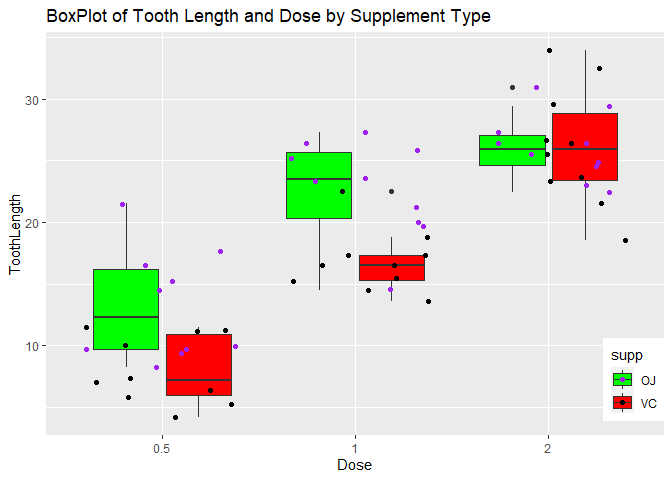
\includegraphics{Project2Inference_files/figure-latex/unnamed-chunk-2-1.pdf}

Let's do Inference print(``is there a correlation between Tooth Length
and supplement type ?'')

\begin{Shaded}
\begin{Highlighting}[]
\KeywordTok{t.test}\NormalTok{(}\DataTypeTok{formula =}\NormalTok{ len }\OperatorTok{\textasciitilde{}}\StringTok{ }\NormalTok{supp , }\DataTypeTok{data =}\NormalTok{ ToothGrowth , }\DataTypeTok{paired =} \OtherTok{FALSE}\NormalTok{ , }\DataTypeTok{var.equal =}\NormalTok{ F )}
\end{Highlighting}
\end{Shaded}

\begin{verbatim}
## 
##  Welch Two Sample t-test
## 
## data:  len by supp
## t = 1.9153, df = 55.309, p-value = 0.06063
## alternative hypothesis: true difference in means is not equal to 0
## 95 percent confidence interval:
##  -0.1710156  7.5710156
## sample estimates:
## mean in group OJ mean in group VC 
##         20.66333         16.96333
\end{verbatim}

Because Our Null Hypothesis is 0 and our p\_value is \textgreater{} 0.05
and the confidence interval contain the 0 , thus we can say there is no
correlation between the supplement type,but is that true ? .

Let's do another Inference print(``is there a correlation between Tooth
Length and Supplement type based on dose level ?'')

\begin{Shaded}
\begin{Highlighting}[]
\NormalTok{ToothGrowth}\OperatorTok{$}\NormalTok{dose}
\end{Highlighting}
\end{Shaded}

\begin{verbatim}
##  [1] 0.5 0.5 0.5 0.5 0.5 0.5 0.5 0.5 0.5 0.5 1   1   1   1   1   1   1   1   1  
## [20] 1   2   2   2   2   2   2   2   2   2   2   0.5 0.5 0.5 0.5 0.5 0.5 0.5 0.5
## [39] 0.5 0.5 1   1   1   1   1   1   1   1   1   1   2   2   2   2   2   2   2  
## [58] 2   2   2  
## Levels: 0.5 1 2
\end{verbatim}

\begin{Shaded}
\begin{Highlighting}[]
\NormalTok{doselevel05 \textless{}{-}ToothGrowth[ToothGrowth}\OperatorTok{$}\NormalTok{dose }\OperatorTok{==}\StringTok{ "0.5"}\NormalTok{,]}
\NormalTok{doselevel2 \textless{}{-}ToothGrowth[ToothGrowth}\OperatorTok{$}\NormalTok{dose }\OperatorTok{==}\StringTok{ "2"}\NormalTok{,]}
\NormalTok{doselevel1  \textless{}{-}ToothGrowth[ToothGrowth}\OperatorTok{$}\NormalTok{dose }\OperatorTok{==}\StringTok{ "1"}\NormalTok{,]}
\KeywordTok{t.test}\NormalTok{(}\DataTypeTok{formula =}\NormalTok{ len }\OperatorTok{\textasciitilde{}}\StringTok{ }\NormalTok{supp , }\DataTypeTok{data =}\NormalTok{ doselevel05 , }\DataTypeTok{paired =}\NormalTok{ F , }\DataTypeTok{var.equal =}\NormalTok{ F)}
\end{Highlighting}
\end{Shaded}

\begin{verbatim}
## 
##  Welch Two Sample t-test
## 
## data:  len by supp
## t = 3.1697, df = 14.969, p-value = 0.006359
## alternative hypothesis: true difference in means is not equal to 0
## 95 percent confidence interval:
##  1.719057 8.780943
## sample estimates:
## mean in group OJ mean in group VC 
##            13.23             7.98
\end{verbatim}

Wait the confidence interval does not contain 0 , which mean there is a
correlation here between supplement type and tooth length , so i guess
the Dose taken seems to affect the tooth length

\begin{Shaded}
\begin{Highlighting}[]
\KeywordTok{t.test}\NormalTok{(}\DataTypeTok{formula =}\NormalTok{ len }\OperatorTok{\textasciitilde{}}\StringTok{ }\NormalTok{supp , }\DataTypeTok{data =}\NormalTok{ doselevel1 , }\DataTypeTok{paired =}\NormalTok{ F , }\DataTypeTok{var.equal =}\NormalTok{ F)}
\end{Highlighting}
\end{Shaded}

\begin{verbatim}
## 
##  Welch Two Sample t-test
## 
## data:  len by supp
## t = 4.0328, df = 15.358, p-value = 0.001038
## alternative hypothesis: true difference in means is not equal to 0
## 95 percent confidence interval:
##  2.802148 9.057852
## sample estimates:
## mean in group OJ mean in group VC 
##            22.70            16.77
\end{verbatim}

Wait the confidence interval does not contain 0 , which mean there is a
correlation here between supplement type and tooth length ,it could be
affect the length of Tooth , so i guess the Dose taken seems to affect
the tooth length

\begin{Shaded}
\begin{Highlighting}[]
\KeywordTok{t.test}\NormalTok{(}\DataTypeTok{formula =}\NormalTok{ len }\OperatorTok{\textasciitilde{}}\StringTok{ }\NormalTok{supp , }\DataTypeTok{data =}\NormalTok{ doselevel2 , }\DataTypeTok{paired =}\NormalTok{ F , }\DataTypeTok{var.equal =}\NormalTok{ F) }
\end{Highlighting}
\end{Shaded}

\begin{verbatim}
## 
##  Welch Two Sample t-test
## 
## data:  len by supp
## t = -0.046136, df = 14.04, p-value = 0.9639
## alternative hypothesis: true difference in means is not equal to 0
## 95 percent confidence interval:
##  -3.79807  3.63807
## sample estimates:
## mean in group OJ mean in group VC 
##            26.06            26.14
\end{verbatim}

Ahh We Found it , seems this guy here doesnt correlated the tooth length
,for given people with high Dose level

\hypertarget{assumptions-needed-for-the-conclusions}{%
\subsection{Assumptions Needed For The
Conclusions:}\label{assumptions-needed-for-the-conclusions}}

\begin{itemize}
\tightlist
\item
  Members of the sample population, the 60 guinea pigs, are
  representative of the entire population of guinea pigs. This
  assumption Satisfied The Random Sample.
\item
  For Each P and (p-1) is exactly \textgreater= 10 are satisfied to
\end{itemize}

For the t-tests, the variances are assumed to be different for the two
groups being compared. This assumption is less stronger than the case in
which the variances are assumed to be equal.

\hypertarget{conclusion}{%
\subsection{\# Conclusion}\label{conclusion}}

\begin{itemize}
\tightlist
\item
  is Dose Level affected taken affecting the result ? Yes, Increase in
  supplement Dose levels leads to overall increase in Tooth length on
  average.
\end{itemize}

-is there a correlation between Tooth Length supplement type by the dose
level ? Yes ,Supplement method has no significant impact on Tooth length
for doseLevel 2 ,but for doselevel 0.5 and 1 it seems there are a
significant impact.

-"which is better for tooth length growth?Orange Juice increase a tooth
length growth more fast compare the ascorbic acid

\end{document}
